\section{CIE 1931-XYZ空间}
题目中第二个任务为画出色品图,并在其上面画出LED RGB三色灯所组成的色域维度,并与NTSC色域进行对比,给出百分比定量结论。首先我们实现色品图,其原理与上一节的一样,将波长单色光转化为范围约束线,坐标转换为sRGB颜色,基本流程与上一节大同小异。

\subsection{CIE 1931-XYZ空间 -- 色品图}

色品图的绘制关键在于限定马蹄的边缘以及图上的每一点,从上一节我们得知可见光XYZ值是如何得来的\eqref{eq:wavelength2xyz}。因此我们得到了每个波长的XYZ,根据公式\eqref{eq:tri-xyz-n}我们便可以得到每个波长在色品图中的坐标点。如图\ref{fig:sd1931edges}所示。

\begin{figure}[htbp]
    \centering
    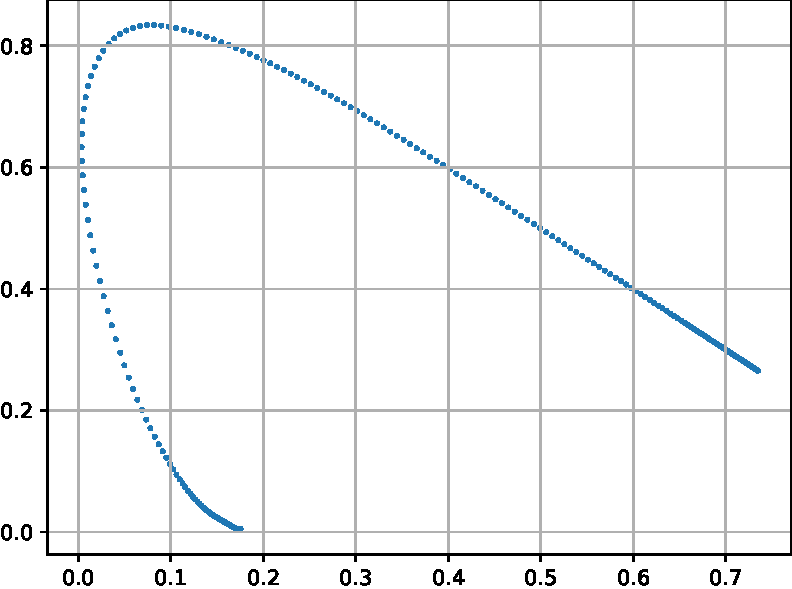
\includegraphics[width=0.65\textwidth]{./imgs/sec3/cd-edge-s.pdf}
    \caption{基于CIE 1931-XYZ的单色光坐标点图}
    \label{fig:sd1931edges}
\end{figure}

从图中我们获取了两个信息,一是单色光坐标点图不是一个闭合空间,二是可见单色光对应的横纵坐标都是在$0\sim1$之间的。针对第一个信息所带来的问题,我们将380nm与780nm对应的单色光的两点使用一条直线连接起来,最终效果如图\ref{fig:sd1931edge}所示。

\begin{figure}[htbp]
    \centering
    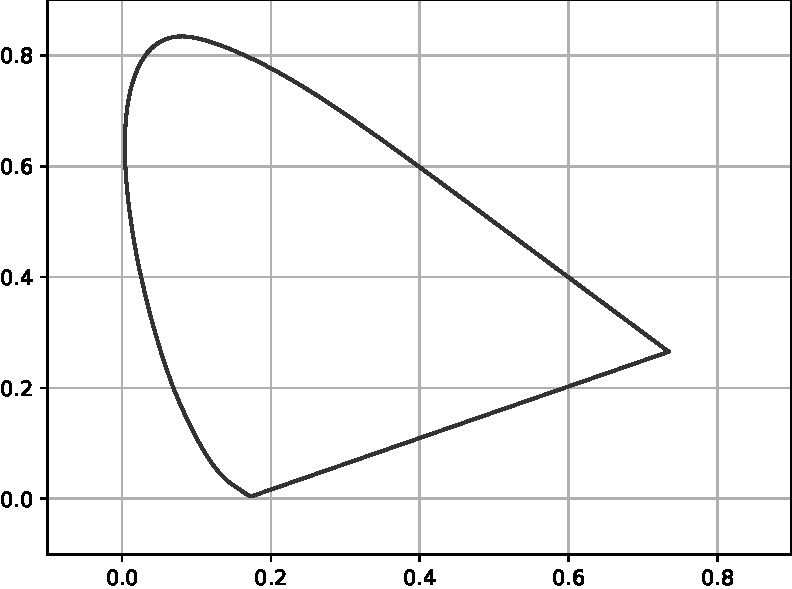
\includegraphics[width=0.65\textwidth]{./imgs/sec3/cd-edge.pdf}
    \caption{基于CIE 1931-XYZ的单色光坐标马蹄图}
    \label{fig:sd1931edge}
\end{figure}

得到了轮廓,下一步就需要得到轮廓内部的每一个坐标点对应的颜色,由于我们所使用的三刺激值并非一个连续的值,如图\ref{fig:sd1931edges}所示,散点图中部分位置有较大的间隔,图\ref{fig:sd1931edge}也是线性化,因此获取轮廓内部的坐标点是较为困难的,因此结合上面获取的第二个信息,做一个偷懒的方法,对$0\sim1$正方形中的每一个点做一个xy转sRGB的操作,详细过程为,根据坐标点和$Y=1$组成xyY系统值,根据公式\eqref{eq:tri-xyz-n}与xyY值我们可以获取到坐标对应的XYZ值,接下来就简单了,使用公式\eqref{eq:trans-xyz2srgb}将XYZ转为sRGB值,这个值就是坐标点的颜色,最终效果图如图\ref{fig:sd1931bgtotal}所示。

\begin{figure}[htbp]
    \centering
    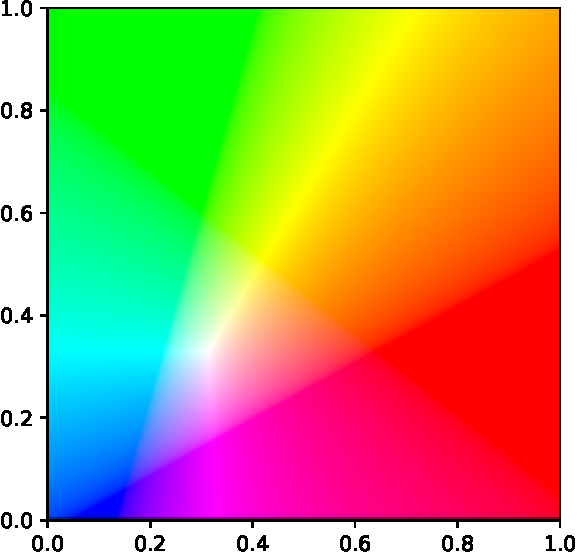
\includegraphics[width=0.65\textwidth]{./imgs/sec3/cd-bg01.pdf}
    \caption{基于CIE 1931-XYZ的颜色背景图}
    \label{fig:sd1931bgtotal}
\end{figure}

相比与前面光谱而言,我们这里少了一步白光自适应的操作,这里我也是借鉴了Colour的思路,它认为XYZ的马蹄图中参考白光为D65,而光谱中的参考白光是E,需要转换到D65。因此在马蹄图的绘制中我们也没有做色度自适应的操作(白光自适应)。

下一步就是根据图\ref{fig:sd1931edge}中的边缘对图\ref{fig:sd1931bgtotal}进行区域限制,再加上一些刻度信息,便可以完成了马蹄图的背景部分了,一个色品图便出现了,效果如图\ref{fig:sd1931}所示。

\begin{figure}[htbp]
    \centering
    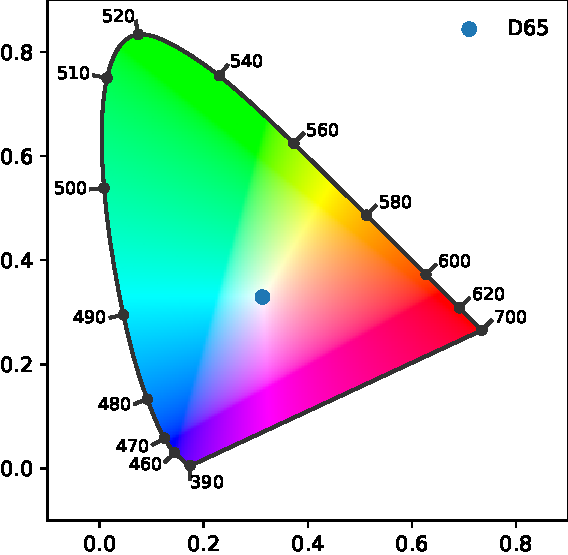
\includegraphics[width=0.65\textwidth]{./imgs/sec3/cd-bg.pdf}
    \caption{基于CIE 1931-XYZ的色品图}
    \label{fig:sd1931}
\end{figure}


\subsection{绘制CIE 1931-XYZ空间色域}

数据同上一节一样,接下来的操作也比较简单,只需录入数据,使用使用原始公式求和\eqref{eq:tri-xyz}得到XYZ,使用公式\eqref{eq:tri-xyz-n}获取xy点以及公式\eqref{eq:trans-xyz2srgb}获取RGB信息。流程为:
\begin{itemize}
    \item [1. ]导入光谱数据与三刺激值数据
    \item [2. ](选做)对三刺激值数据做白光自适应\eqref{eq:CAT},的光谱数据通道归一化
    \item [3. ]光谱数据与变换过后的三刺激值数据求和,对$Y$做归一化处理\eqref{eq:tri-xyz},根据公式\eqref{eq:tri-xyz-n}获取xy点,公式\eqref{eq:trans-xyz2srgb}获取RGB信息
    \item [4. ]将xy与RGB信息对应绘制到图上
\end{itemize}
最终效果如图\ref{fig:sd1931-led}所示。

\begin{figure}[htbp]
    \centering
    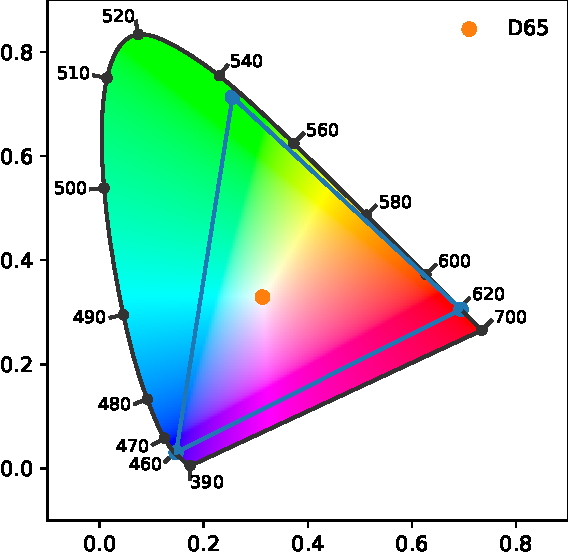
\includegraphics[width=0.65\textwidth]{./imgs/sec3/cd-led.pdf}
    \caption{LED色域}
    \label{fig:sd1931-led}
\end{figure}

美国国家电视标准委员会(National Television Standards Committee,NTSC)在1952年制定了彩色电视广播标准,包括了NTSC色域的定义,NTSC色域在XYZ色彩空间中,为RGB三色的坐标为$R_{xy}=(0.630, 0.340)$、$G_{xy}=(0.310, 0.595)$、$B_{xy}=(0.155, 0.070)$。本文第二个子目标需要给出以NTSC为基准定量结论,因此我们需要一个计算面积的方式,考虑到第四个基色的实验,本文使用鞋带公式\cite{braden1986surveyor}作为不定形状多边形的计算方式,携带公式如\eqref{eq:Shoelace}所示。

\begin{equation}
    \begin{aligned}
        A &= \lvert\frac 1 2 \sum_{i=1}^n (y_i + y_{i+1})(x_i - x_{i+1})\rvert\\
          &= \frac 1 2 \lvert(y_1+y_2)(x_1-x_2)+ \cdots +(y_n+y_1)(x_n-x_1)\rvert
    \end{aligned}
    \label{eq:Shoelace}
\end{equation}

根据面积计算后,可得图\ref{fig:sd1931-ledwithntsc}。

\begin{figure}[htbp]
    \centering
    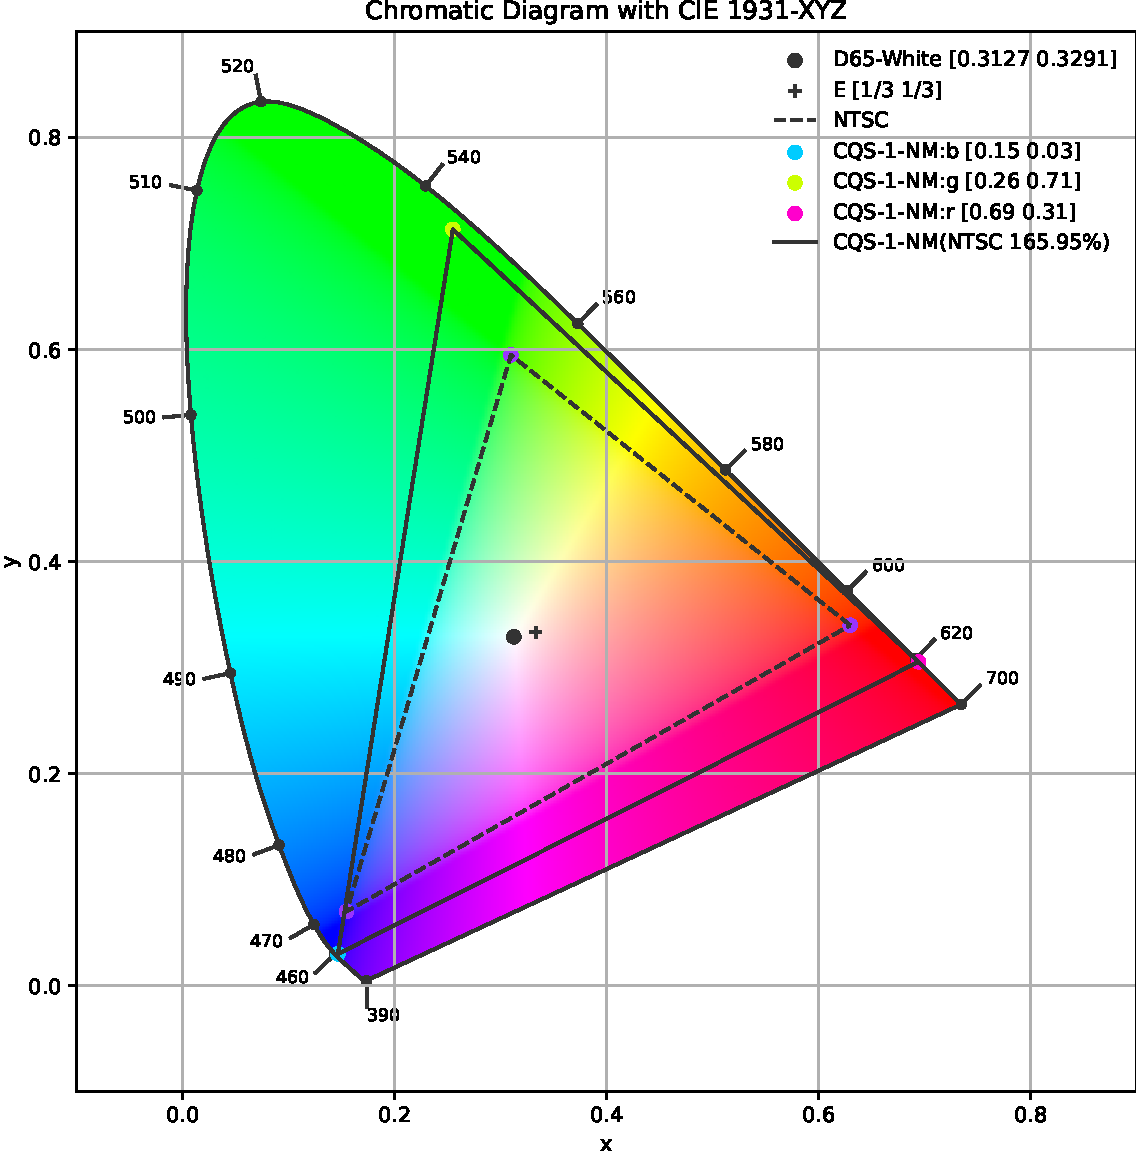
\includegraphics[width=0.65\textwidth]{./imgs/sec3/CQS-1-NM-1931-sd.pdf}
    \caption{CIE 1931-XYZ色彩匹配函数下的LED色域与NTSC色域}
    \label{fig:sd1931-ledwithntsc}
\end{figure}

从图中我们可以获知,我们的RGB LED灯组成的色域是``NTSC 165.95\%''的,就此我们完成了第二个子目标--基于CIE 1931-XYZ空间色品图与色域定量计算。